\subsection{\={O}saka daigaku}

Este experimento corresponde a la Universidad de Osaka, localizada en Osaka, Japón. Más especificamente, nuestro traceroute es al departamento de Ciencias de la Computación de la Universidad de Osaka, que se encuentra en la dirección \url{www.es.osaka-u.ac.jp}.

\begin{figure}[H]
    \centering
    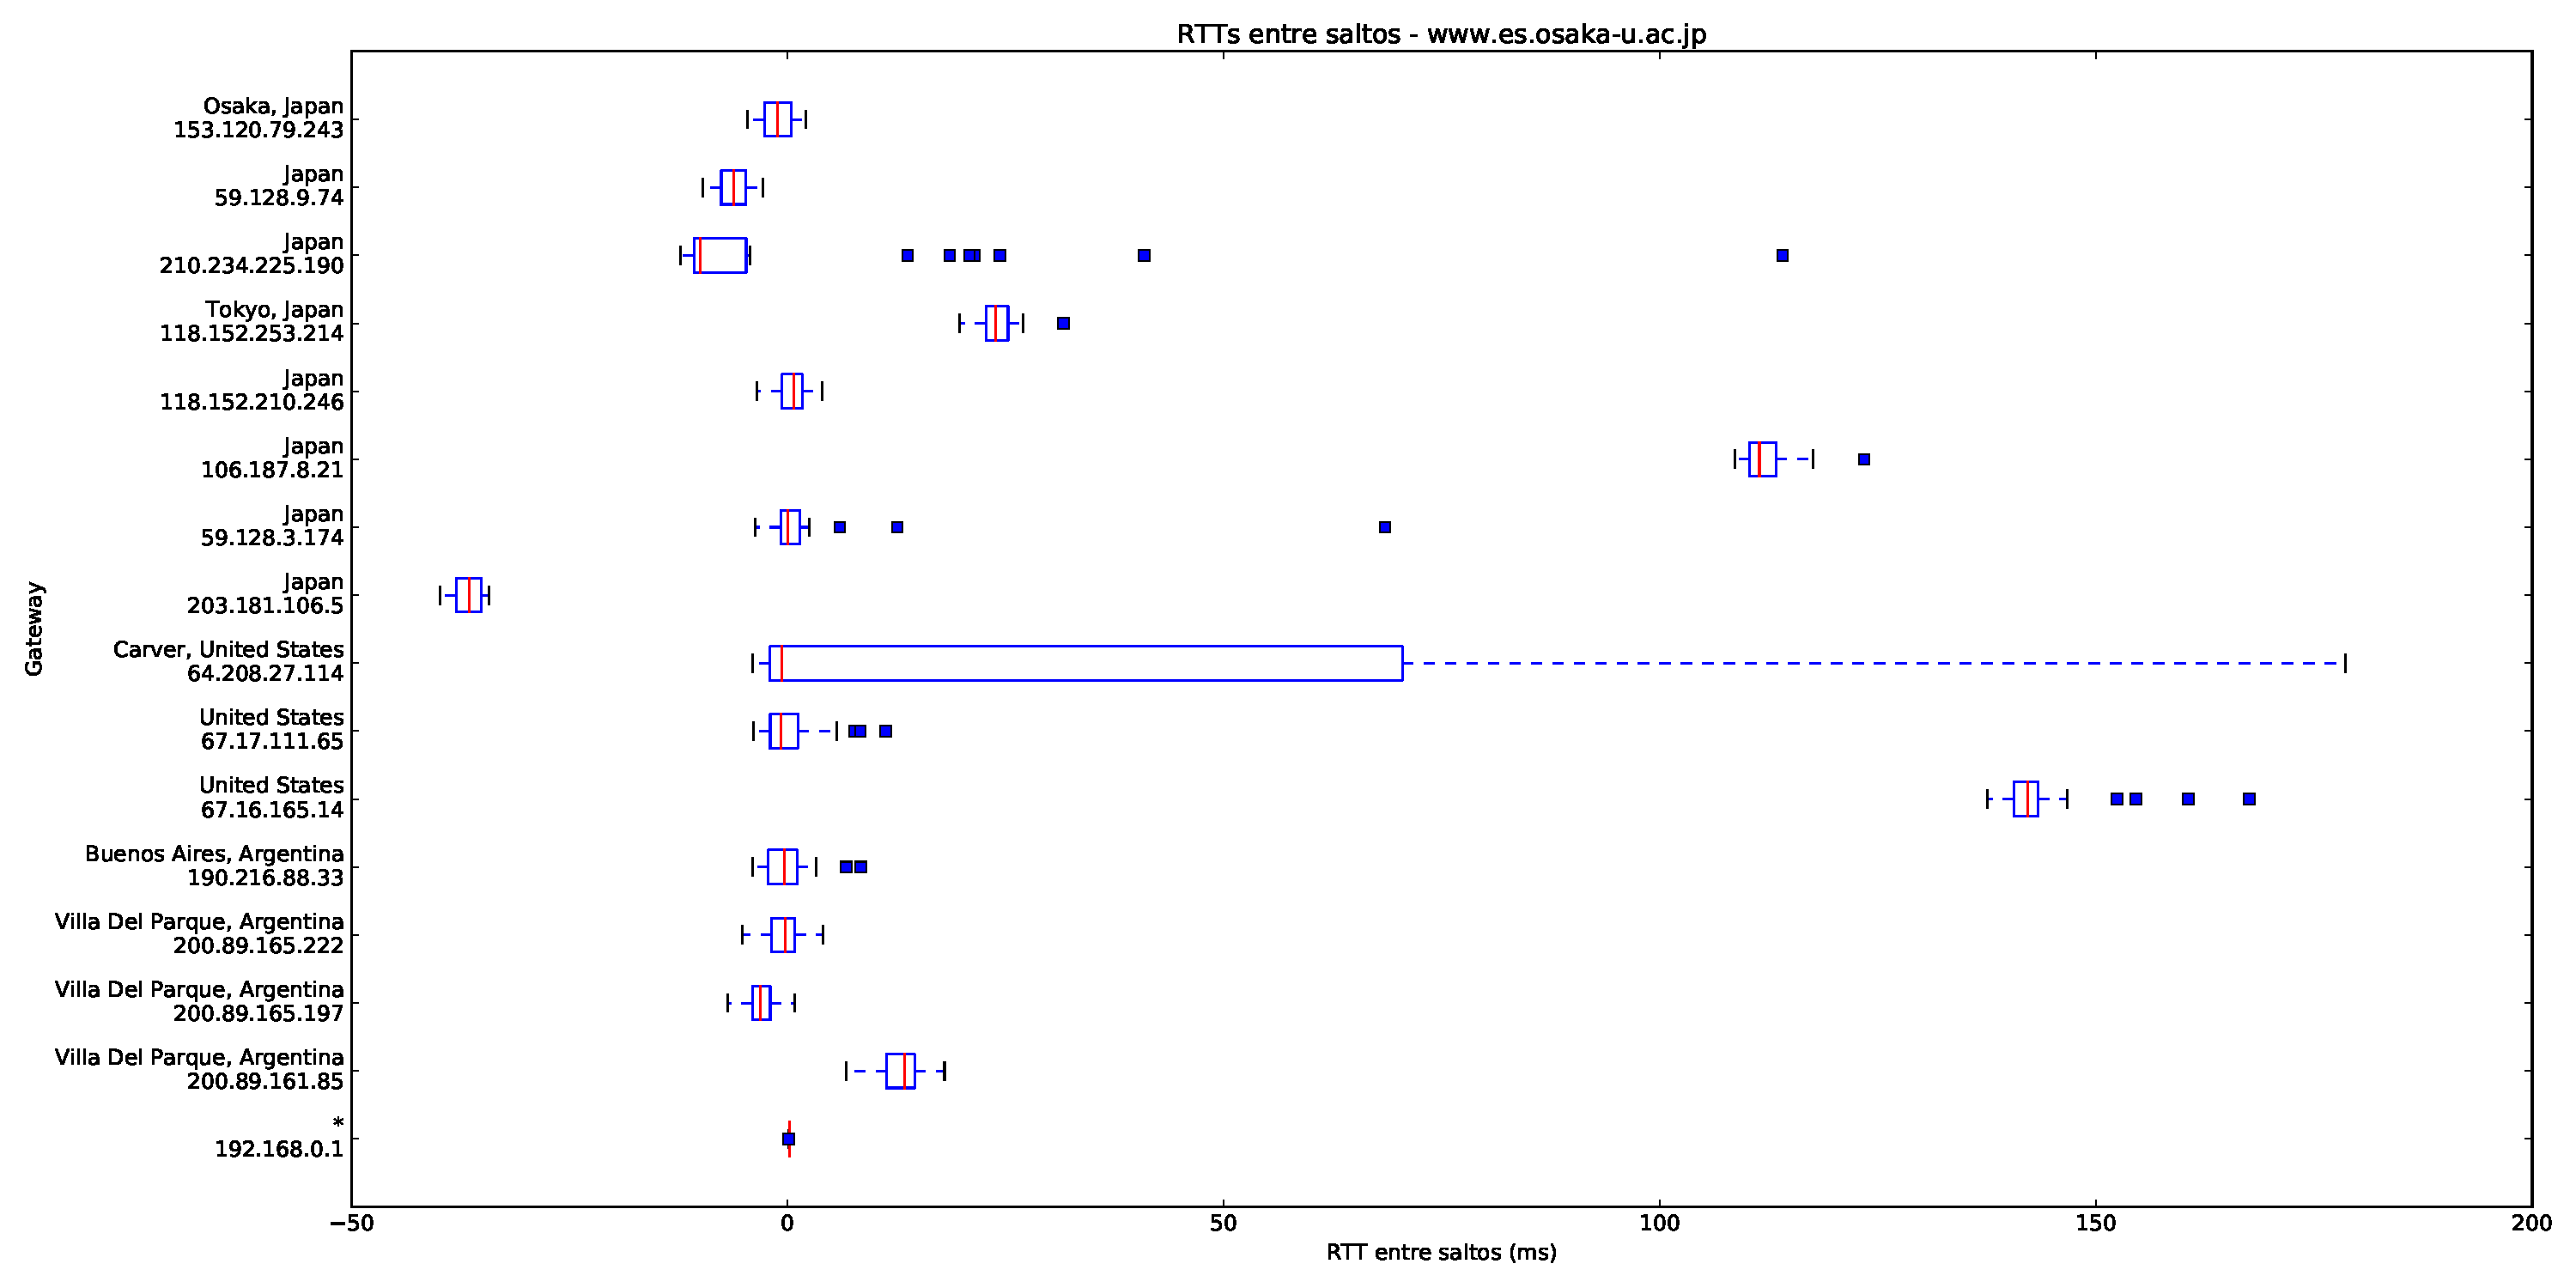
\includegraphics[width=8.5cm]{img/grafico1-www-es-osaka-u-ac-jp.pdf}
    \caption{\normalfont RTTs entre saltos. El valor asignado al $i$-ésimo nodo corresponde al salto entre el $i$-ésimo y el $i - 1$-ésimo nodo. Para el primer nodo se utiliza simplemente su RTT.}
\end{figure}

Se observan mediciones normales que explicaremos a continuación. En el gateway de Craver, Estados Unidos observamos algunas mediciones con un promedio muy alto. Tomamos las mediciones varias veces y siempre daba así. Se lo podemos atribuir a que quizás el gateway estaba muy sobrecargado en ese momento, dado que probamos varios días después y ya no sucedía.

\begin{figure}[H]
    \centering
    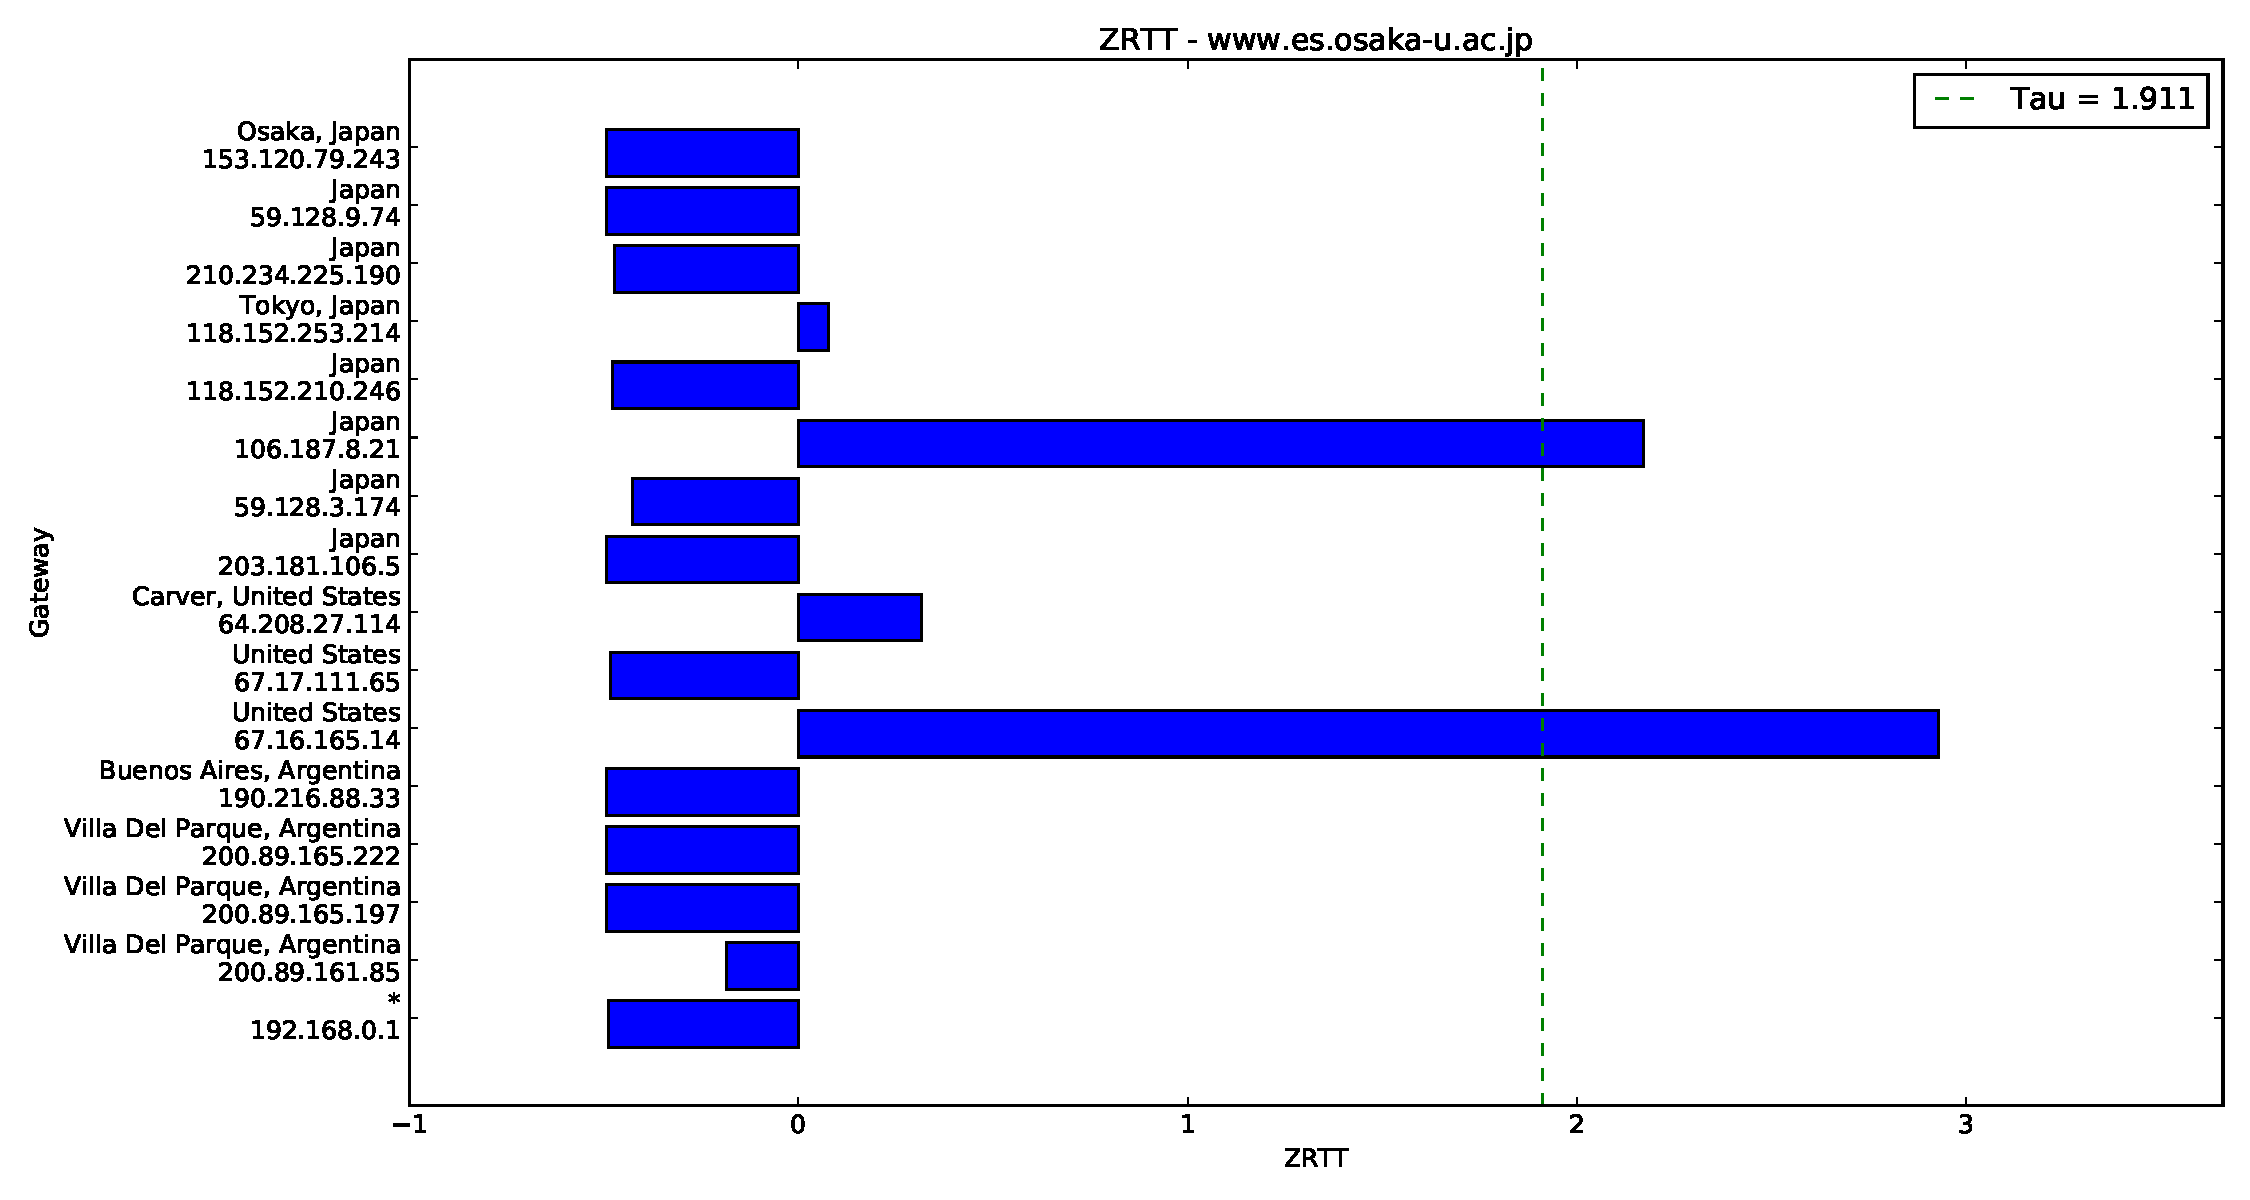
\includegraphics[width=8.5cm]{img/grafico2-www-es-osaka-u-ac-jp.pdf}
    \caption{\normalfont ZRTTs entre saltos.}
\end{figure}

Sin embargo, en el gráfico de $ZRTT$ podemos observar problemas con la geolocalización IP. Hay 2 IPs en la ruta que nos indican que el gateway está en Japón, pero recién el tercero está indicado como un enlace intercontinental.
Esto nos permite afirmar, con bastante seguridad, que las dos primeras IP que según el servicio de geolocalización IP están en Japón (\texttt{203.181.106.5} y \texttt{59.128.3.174}), están en realidad en Estados Unidos.

El porcentaje de saltos que no responden los time exceeded es 30.43\% (exactamente 7 de 23). En términos de saltos que sí responden, la ruta tiene 16 nodos, incluyendo nuestro router.

\begin{figure}[H]
    \centering
    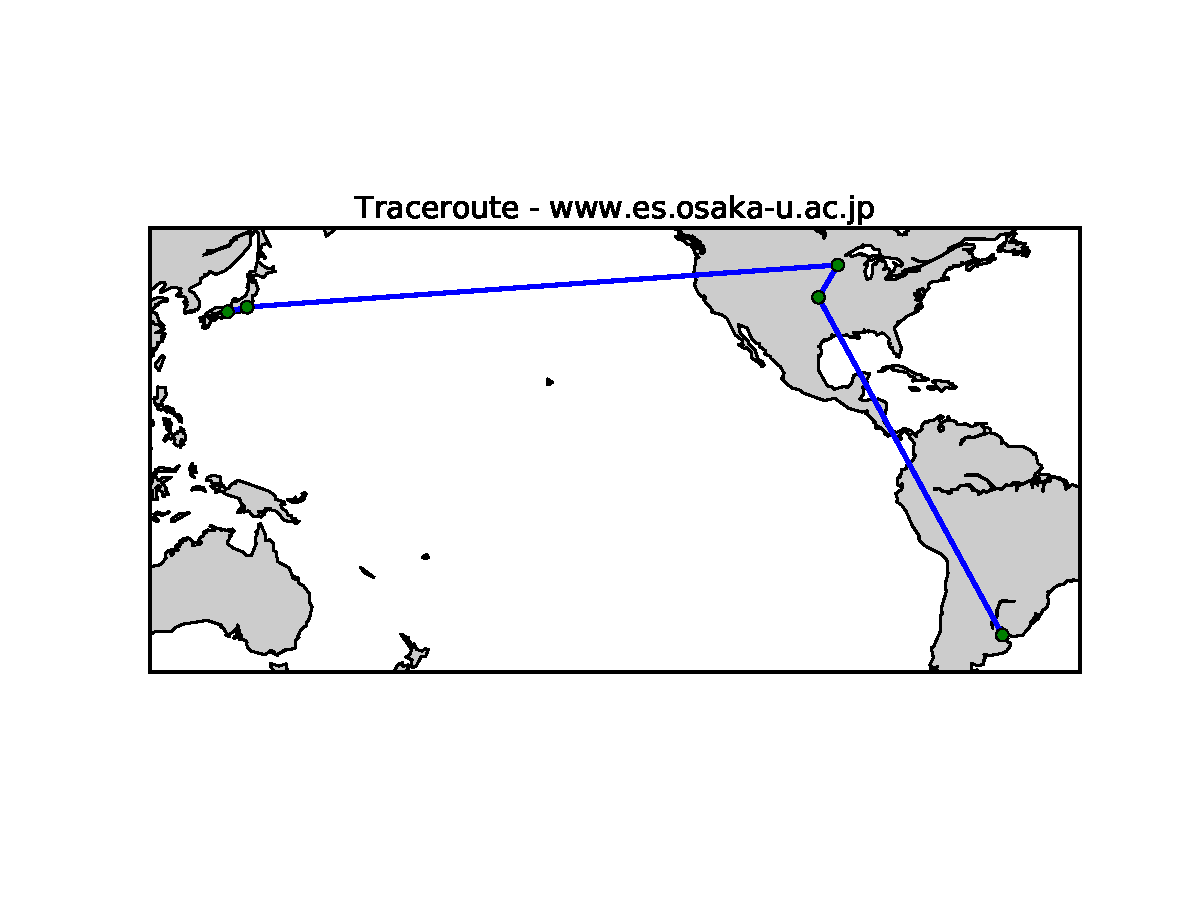
\includegraphics[width=8.5cm]{img/grafico3-www-es-osaka-u-ac-jp.pdf}
    \caption{\normalfont Ubicación geográfica estimada de la ruta tomada.}
\end{figure}


Como se ve, la ruta es aproximadamente la esperada. La ruta como bien se observa en el mapa, tiene 2 saltos intercontinentales, y como bien predijo nuestro modelo, tiene 2 enlaces submarinos, uno entre Argentina y Estados Unidos, y otro entre Estados Unidos y Japón.

En este caso el modelo fue extremadamente preciso: hay 2 enlaces submarinos y nuestro modelo los detectó, y no detectó ninguno más (es decir, no hubo falsos negativos).



